\documentclass{article}
\usepackage[utf8]{inputenc}
\usepackage{amsmath}
\usepackage{amssymb}
\usepackage{amsfonts}
\usepackage{graphicx}
\usepackage{tikz}
\usetikzlibrary{angles,fit,arrows,calc,math,matrix,intersections,through,backgrounds,cd}
\usepackage{pgfplots}
\pgfplotsset{compat=1.18}
\usepackage{geometry}
\geometry{a4paper, margin=1in}
\usepackage{booktabs} % For professional looking tables

\title{Visualization and Analysis of $4_1$ Knot Paths in (U,V) Space and $e^V$ Weighted Area}
\author{Manus}
\date{\today}

\begin{document}
\maketitle

\section{Introduction}
This document explores the second research direction: the visualization and preliminary analysis of geometric properties of paths associated with the figure-eight knot ($4_1$) within the $(U,V)$ reference space. A key focus is understanding the $e^V$ weighted area, which arises in the geometric interpretation of global arithmetic torsion, $\mathcal{T}(S) = \iint_{\Sigma_S} e^V dV \wedge dU$.

The $4_1$ knot (Figure-Eight Knot) is the simplest hyperbolic knot and serves as a fundamental example for exploring connections between knot theory and Arithmetic Expression Geometry (AEG).

\begin{figure}[h!]
    \centering
    \documentclass{standalone}
\usepackage{amsthm}
\usepackage{amssymb}
\usepackage{amsfonts}
\usepackage{amsmath}
\usepackage{mathtools}

\usepackage{pgf}
\usepgflibrary{fpu}
\usepackage{pgfplots}
\usepackage{tikz}
\usetikzlibrary{angles,fit,arrows,calc,math,matrix,intersections,through,backgrounds,cd}
\usepackage{tkz-euclide}
\usepackage{tkz-graph}
\usepackage{graphicx}
\pgfplotsset{compat=1.18}

\begin{document}

        \tikzmath{
                \one = 1;
                \base = 2.618033988749;
                \offset = 15.8888888;
                \valofpi = 3.1415926;
                \anglei = 3.1415926;
                \angleo = 3.1415926;
        }

        \begin{tikzpicture}[scale=1.0]
                % 1. 绘制坐标轴
                \draw[black, line width=0.6pt, ->]
                (\offset,0) to[out=90,in=270] (\offset,15.5)
                node [anchor=south] {y};

                \draw[black, line width=0.6pt, ->]
                (-7.5,0) to[out=0,in=180] (18,0)
                node [anchor=west] {x};

                % 2. 绘制 x 和 y 坐标轴刻度
                \foreach \x in {-25,...,2} {
                        \node [anchor=north] at (\x/9*8 + \offset, 0) {\x};
                }
                \foreach \y in {1,...,17} {
                        \node [anchor=-135] at (18, \y/9*8) {\y};
                }

                % 3. 浅灰色水平网格线
                \foreach \t in {17,...,1} {
                        \draw [lightgray, line width=0.6pt]
                        (-7.5,\t/9*8)
                        to[out=0,in=180]
                        (18,\t/9*8);
                }

                % 4. 浅灰色竖直网格线
                \foreach \t in {-26,...,2} {
                        \draw [lightgray, line width=0.6pt]
                        (\t/9*8 + \offset, 0)
                        to[out=90,in=270]
                        (\t/9*8 + \offset, 15.5);
                }




        \end{tikzpicture}
\end{document}

    \caption{The Figure-Eight Knot ($4_1$).}
    \label{fig:knot_4_1_q2}
\end{figure}

\section{Geometric Interpretation of Arithmetic Torsion}
Material 5 of the provided research background introduces a geometric interpretation of the global arithmetic torsion for a path $S$ (typically a relator in the knot group $G(K)$) as an integral over a surface $\Sigma_S$ in a $(U,V)$ reference space:
\[
\mathcal{T}(S) = \iint_{\Sigma_S} e^V dV \wedge dU
\]
Here, $U$ and $V$ are coordinates in a 2-dimensional space where arithmetic operations of addition and multiplication are represented as translations. For an arithmetic expression $P$, $U(P)$ can be thought of as related to the additive structure and $V(P)$ to the multiplicative structure. Specifically, if an expression involves $m$ multiplications by a factor $t_k$ at each step, $V$ can accumulate as $V = \sum \ln t_k$. If $t$ is a constant parameter for $m$ multiplicative operations, $V = m \ln t$.

\section{Visualizing Paths and Enclosed Areas in (U,V) Space}

\subsection{Plotting Paths}
To analyze the geometric torsion, paths corresponding to relators of $G(4_1)$ are plotted in the $(U,V)$ plane. Each segment of the path is determined by the arithmetic operations (e.g., $\oplus_c$ or $\otimes_t$) in the relator word. For a relator $S$, its path starts at the origin $(0,0)$ and, by definition of a relator, should end at a point that is identified with the origin in the context of the AEG space (though the $(U,V)$ coordinates themselves might not return to $(0,0)$ if there's a non-trivial $K$ value, which corresponds to a deck transformation).

The path $S$ and its reverse path $S_{\text{rev}}$ (or a path that closes the loop appropriately) define the boundary of the surface $\Sigma_S$.

\begin{figure}[h!]
    \centering
    \resizebox{0.8\textwidth}{!}{\documentclass{standalone}
\usepackage{amsmath}
\usepackage{tikz}

\begin{document}
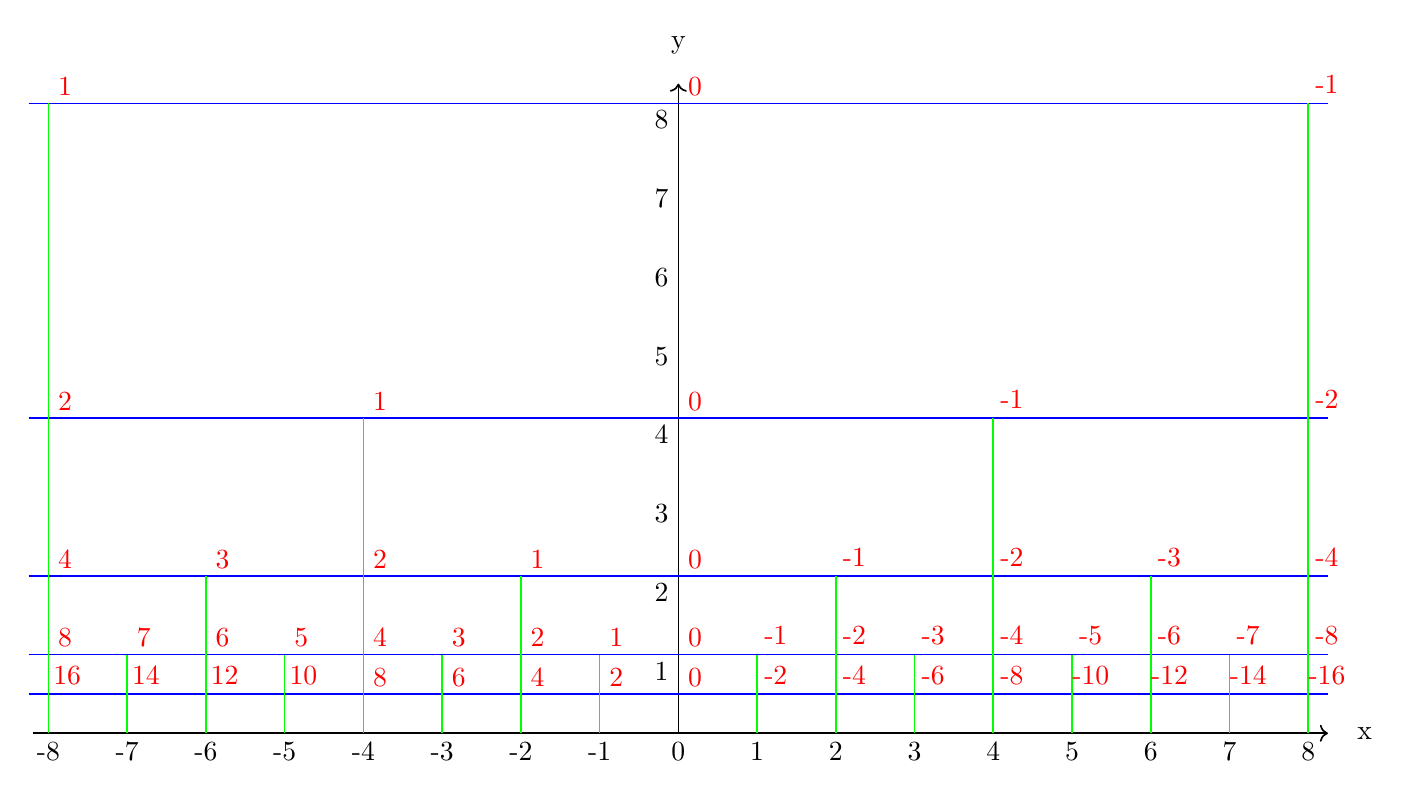
\begin{tikzpicture}
\draw [black, line width=0.6pt, ->] (0,0) to[out=90,in=270] (0,8.25);
\node [anchor=south] at (0,8.5) {y};
\draw [black, line width=0.6pt, ->] (-8.2,0) to[out=0,in=180] (8.25,0);
\node [anchor=west] at (8.5,0) {x};
\foreach \x in {-8,-7,-6,-5,-4,-3,-2,-1,0,1,2,3,4,5,6,7,8}
  \node [anchor=north] at (\x,0) {\x};
\foreach \y in {1,2,3,4,5,6,7,8}
  \node [anchor=45] at (0,\y) {\y};

\draw [blue, line width=0.6pt] (-8.25,0.5) to[out=0,in=180] (8.25,0.5);
\draw [blue, line width=0.6pt] (-8.25,1) to[out=0,in=180] (8.25,1);
\draw [blue, line width=0.6pt] (-8.25,2) to[out=0,in=180] (8.25,2);
\draw [blue, line width=0.6pt] (-8.25,4) to[out=0,in=180] (8.25,4);
\draw [blue, line width=0.6pt] (-8.25,8) to[out=0,in=180] (8.25,8);

\draw [green, line width=0.6pt] (-8,0) to[out=90,in=270] (-8,1);
\draw [green, line width=0.6pt] (-7,0) to[out=90,in=270] (-7,1);
\draw [green, line width=0.6pt] (-6,0) to[out=90,in=270] (-6,1);
\draw [green, line width=0.6pt] (-5,0) to[out=90,in=270] (-5,1);
\draw [green, line width=0.6pt] (-4,0) to[out=90,in=270] (-4,1);
\draw [green, line width=0.6pt] (-3,0) to[out=90,in=270] (-3,1);
\draw [green, line width=0.6pt] (-2,0) to[out=90,in=270] (-2,1);
\draw [green, line width=0.6pt] (-1,0) to[out=90,in=270] (-1,1);
\draw [green, line width=0.6pt] (1,0) to[out=90,in=270] (1,1);
\draw [green, line width=0.6pt] (2,0) to[out=90,in=270] (2,1);
\draw [green, line width=0.6pt] (3,0) to[out=90,in=270] (3,1);
\draw [green, line width=0.6pt] (4,0) to[out=90,in=270] (4,1);
\draw [green, line width=0.6pt] (5,0) to[out=90,in=270] (5,1);
\draw [green, line width=0.6pt] (6,0) to[out=90,in=270] (6,1);
\draw [green, line width=0.6pt] (7,0) to[out=90,in=270] (7,1);
\draw [green, line width=0.6pt] (8,0) to[out=90,in=270] (8,1);

\draw [green, line width=0.6pt] (-8,1) to[out=90,in=270] (-8,2);
\draw [green, line width=0.6pt] (-6,1) to[out=90,in=270] (-6,2);
\draw [green, line width=0.6pt] (-4,1) to[out=90,in=270] (-4,2);
\draw [green, line width=0.6pt] (-2,1) to[out=90,in=270] (-2,2);
\draw [green, line width=0.6pt] (2,1) to[out=90,in=270] (2,2);
\draw [green, line width=0.6pt] (4,1) to[out=90,in=270] (4,2);
\draw [green, line width=0.6pt] (6,1) to[out=90,in=270] (6,2);
\draw [green, line width=0.6pt] (8,1) to[out=90,in=270] (8,2);

\draw [green, line width=0.6pt] (-8,2) to[out=90,in=270] (-8,4);
\draw [green, line width=0.6pt] (-4,2) to[out=90,in=270] (-4,4);
\draw [green, line width=0.6pt] (4,2) to[out=90,in=270] (4,4);
\draw [green, line width=0.6pt] (8,2) to[out=90,in=270] (8,4);

\draw [green, line width=0.6pt] (-8,4) to[out=90,in=270] (-8,8);
\draw [green, line width=0.6pt] (8,4) to[out=90,in=270] (8,8);

\node [anchor=225, red] at (-8,0.5) {16};
\node [anchor=225, red] at (-7,0.5) {14};
\node [anchor=225, red] at (-6,0.5) {12};
\node [anchor=225, red] at (-5,0.5) {10};
\node [anchor=225, red] at (-4,0.5) {8};
\node [anchor=225, red] at (-3,0.5) {6};
\node [anchor=225, red] at (-2,0.5) {4};
\node [anchor=225, red] at (-1,0.5) {2};
\node [anchor=225, red] at (0,0.5) {0};
\node [anchor=225, red] at (1,0.5) {-2};
\node [anchor=225, red] at (2,0.5) {-4};
\node [anchor=225, red] at (3,0.5) {-6};
\node [anchor=225, red] at (4,0.5) {-8};
\node [anchor=225, red] at (5,0.5) {-10};
\node [anchor=225, red] at (6,0.5) {-12};
\node [anchor=225, red] at (7,0.5) {-14};
\node [anchor=225, red] at (8,0.5) {-16};

\node [anchor=225, red] at (-8,1) {8};
\node [anchor=225, red] at (-7,1) {7};
\node [anchor=225, red] at (-6,1) {6};
\node [anchor=225, red] at (-5,1) {5};
\node [anchor=225, red] at (-4,1) {4};
\node [anchor=225, red] at (-3,1) {3};
\node [anchor=225, red] at (-2,1) {2};
\node [anchor=225, red] at (-1,1) {1};
\node [anchor=225, red] at (0,1) {0};
\node [anchor=225, red] at (1,1) {-1};
\node [anchor=225, red] at (2,1) {-2};
\node [anchor=225, red] at (3,1) {-3};
\node [anchor=225, red] at (4,1) {-4};
\node [anchor=225, red] at (5,1) {-5};
\node [anchor=225, red] at (6,1) {-6};
\node [anchor=225, red] at (7,1) {-7};
\node [anchor=225, red] at (8,1) {-8};

\node [anchor=225, red] at (-8,2) {4};
\node [anchor=225, red] at (-6,2) {3};
\node [anchor=225, red] at (-4,2) {2};
\node [anchor=225, red] at (-2,2) {1};
\node [anchor=225, red] at (0,2) {0};
\node [anchor=225, red] at (2,2) {-1};
\node [anchor=225, red] at (4,2) {-2};
\node [anchor=225, red] at (6,2) {-3};
\node [anchor=225, red] at (8,2) {-4};

\node [anchor=225, red] at (-8,4) {2};
\node [anchor=225, red] at (-4,4) {1};
\node [anchor=225, red] at (0,4) {0};
\node [anchor=225, red] at (4,4) {-1};
\node [anchor=225, red] at (8,4) {-2};

\node [anchor=225, red] at (-8,8) {1};
\node [anchor=225, red] at (0,8) {0};
\node [anchor=225, red] at (8,8) {-1};

\end{tikzpicture}
\end{document}
}
    \caption{Conceptual visualization of a path $S$ in the $(U,V)$ reference space. The path traces a trajectory based on arithmetic operations, and a closed loop (formed by $S$ and potentially $S_{\text{rev}}$ or other segments) encloses the region $\Sigma_S$.}
    \label{fig:uv_path_q2}
\end{figure}

Figure \ref{fig:uv_path_q2} provides a conceptual illustration of such a path. For specific $4_1$ relators, these paths would be explicitly constructed based on the chosen arithmetic interpretation (e.g., $a \mapsto \otimes_t, b \mapsto \oplus_1$).

\subsection{The Weighting Factor $e^V$}
The term $e^V$ acts as a weighting factor for the area element $dV \wedge dU$. Since $V$ represents the accumulated effect of multiplications, $e^V$ can be seen as $e^{\sum \ln t_k} = \prod t_k$. This means the contribution of an area element to the torsion integral is scaled by the product of the multiplicative factors encountered along the path to reach that region.

Visualizing the $e^V$ field over the $(U,V)$ plane (or at least over the region $\Sigma_S$) would involve showing how this weighting varies. For example, if $t > 1$, regions with higher $V$ (more multiplications or larger $t_k$) will have exponentially larger weights.

\section{Analysis and Verification}

\subsection{Calculating Weighted Area}
For simple paths $S$ from $G(4_1)$, the weighted area $\iint_{\Sigma_S} e^V dV \wedge dU$ can be estimated or, in some cases, calculated analytically (perhaps with the aid of symbolic computation software like Mathematica or SymPy). This involves:
\begin{enumerate}
    \item Parameterizing the boundary of $\Sigma_S$.
    \item Applying Green's theorem or direct integration, taking into account the $e^V$ factor which depends on the $V$ coordinate.
\end{enumerate}

\subsection{Verification of the Triple Identity}
The calculated geometric torsion can then be compared with the algebraically defined torsion $\Delta(t)(t^K-1)$. This comparison serves as a direct verification of the proposed triple identity (algebraic, geometric, and potentially physical interpretations of torsion) for specific instances related to the $4_1$ knot.

\subsection{Special Case: K=0}
When $K=0$, the algebraic torsion $\mathcal{T}(S)$ becomes zero (assuming $\Delta(t) \neq 0$). This implies that the geometric integral $\iint_{\Sigma_S} e^V dV \wedge dU$ must also be zero. This could occur in several ways:
\begin{itemize}
    \item The unweighted area of $\Sigma_S$ is zero (e.g., the path retraces itself or does not enclose a region).
    \item The $e^V$ weighting is such that positive and negative contributions to the integral cancel out perfectly. This might happen if $\Sigma_S$ has a symmetric shape with respect to the $V$ coordinate, and the $e^V$ weighting leads to cancellations.
\end{itemize}
Visualizing paths for which $K=0$ (identified from the study in Question 1) in the $(U,V)$ space and analyzing their $\Sigma_S$ and $e^V$ distributions would be particularly insightful.

\section{Expected Outcomes}
This investigation is expected to:
\begin{itemize}
    \item Provide concrete visualizations of how paths from $G(4_1)$ map into the $(U,V)$ reference space.
    \item Offer a clearer understanding of how the $e^V$ weighting affects the geometric interpretation of arithmetic torsion.
    \item Allow for preliminary verification of the geometric torsion formula for specific $4_1$ knot relators.
    \item Reveal geometric characteristics of paths or regions $\Sigma_S$ that correspond to $K=0$ or other significant torsion values.
\end{itemize}

This direction aims to solidify the geometric underpinnings of AEG by directly applying its concepts to the $4_1$ knot and visualizing the consequences of its arithmetic interpretation in a geometric space.

\end{document}

